% =====================================================================
%  Section 8.4: Godunov's method.
% =====================================================================

\subsection{Godunov's method}
\label{subsec:godunov}

\subsubsection{The scheme}
\label{subsubsec:godunov-flux}

Let $\mathbb{R}$ be divided into cells $[x_{j-1/2},x_{j+1/2}]$ of width
$\Delta x$, with $t^n=n\Delta t$ and cell averages
$\bar u_j^n=\Delta x^{-1}\int_{x_{j-1/2}}^{x_{j+1/2}}u(x,t^n)\,dx$ approximated by $U_j^n$.
Integrating $u_t+f(u)_x=0$ over a cell and a time step gives
\begin{equation}
  \bar u_j^{n+1} = \bar u_j^n - \frac{\Delta t}{\Delta x}
  \left( F_{j+1/2}^n - F_{j-1/2}^n \right),
  \qquad F_{j+1/2}^n=\frac1{\Delta t}\int_{t^n}^{t^{n+1}}f\big(u(x_{j+1/2},t)\big)\,dt,
\end{equation}
for the exact cell averages $\bar u_j^n$. The scheme replaces $F_{j+1/2}^n$ by a
numerical flux $\widehat f_{j+1/2}$ depending on $U_j^n,U_{j+1}^n$, giving
$U_j^{n+1}=U_j^n-\frac{\Delta t}{\Delta x}(\widehat f_{j+1/2}-\widehat f_{j-1/2})$.
Godunov's method \cite{godunov1959} takes $\widehat f_{j+1/2}$ to be the flux
at $x/t=0$ of the exact Riemann solution with data $(U_j^n,U_{j+1}^n)$
(Theorem~\ref{thm:riemann-solution}):
\begin{equation}
  \label{eq:godunov-flux}
  \widehat f_{j+1/2} = f\big(\omega(0;\, U_j^n, U_{j+1}^n)\big),
\end{equation}
where $\omega(\xi;u_\ell,u_r)$ is the entropy solution with data $(u_\ell,u_r)$ at
$\xi=x/t$. By \eqref{eq:riemann-shock}--\eqref{eq:riemann-rarefaction},
\begin{equation}
  \omega(0; u_\ell,u_r) =
  \begin{cases}
    u_\ell, & u_\ell>u_r,\ \tfrac{u_\ell+u_r}{2}>0, \\
    u_r, & u_\ell>u_r,\ \tfrac{u_\ell+u_r}{2}<0, \\
    u_\ell, & u_\ell\le u_r,\ u_\ell\ge0, \\
    u_r, & u_\ell\le u_r,\ u_r\le0, \\
    0, & u_\ell < 0 < u_r,
  \end{cases}
\end{equation}
the last case corresponding to $\xi=0$ lying inside the fan. If
$u_\ell=-u_r$ the value $\omega(0)$ is ambiguous, but $f(u_\ell)=f(u_r)$, so
\eqref{eq:godunov-flux} is unaffected.

\subsubsection{Stability and convergence}
\label{subsubsec:godunov-convergence}

The scheme is stable and monotone provided the CFL condition
\begin{equation}
  \label{eq:cfl}
  \Delta t \le \frac{\Delta x}{\max_j |U_j^n|}
\end{equation}
holds, which prevents waves from neighbouring interfaces from reaching
$x_{j+1/2}$ within one step \cite[Ch.~4]{leveque2002}.

\begin{theorem}[{\cite[Theorem~1 and \S1]{crandall1980}}]
\label{thm:godunov-convergence}
Let $u_0\in L^1(\mathbb{R})\cap L^\infty(\mathbb{R})$ with $a\le u_0\le b$ a.e.,
and let $\lambda=\Delta t/\Delta x$ be fixed with
$\lambda\max_{a\le u\le b}|f'(u)|\le1$. Let $u^{\Delta}$ be the piecewise
constant function equal to $U_j^n$ on $[x_{j-1/2},x_{j+1/2})\times[t^n,t^{n+1})$,
where $U_j^0$ is the cell average of $u_0$ and the $U_j^n$ are the Godunov
approximations. Then for every $T>0$
\begin{equation*}
  \lim_{\Delta t\to0}\ \sup_{0\le t\le T}\int_{\mathbb{R}}\big|u^{\Delta}(x,t)-u(x,t)\big|\,dx=0,
\end{equation*}
where $u$ is the Kru\v{z}kov entropy solution \cite{kruzhkov1970} with data $u_0$.
\end{theorem}

Crandall and Majda establish this for every consistent conservation-form scheme
that is monotone on $[a,b]$ with Lipschitz continuous numerical flux, and verify
in \S1 that Godunov's scheme for $f''>0$ belongs to this class; the theorem
gives convergence but no rate. For Burgers' equation the Kru\v{z}kov solution
coincides with the Oleinik solution of Theorem~\ref{thm:oleinik-uniqueness}
(standard; see \cite[\S3.4]{evans2010} and \cite{kruzhkov1970}). Since the
Riemann data used below are not in $L^1(\mathbb{R})$, we localise: replacing
them by $0$ outside $[-5,5]$ keeps $u_0$ within $[0,1]$ and, because $|u|\le1$,
leaves the exact solution on $[-2,2]\times[0,1]$ unchanged. At $\lambda=0.45$ the
numerical domain of dependence over $t\le1$ has half-width at most
$t/\lambda<2.23$, so the dependence interval of $[-2,2]$ lies within
$[-4.23,4.23]\subset[-5,5]$ and the computed solution is unchanged as well.
In the experiments $\max_j|U_j^n|=1$ throughout, so the adaptive step
$\Delta t=0.45\,\Delta x/\max_j|U_j^n|$ gives the constant $\lambda=0.45$
required by the theorem (the final step, shortened to land on $t=1$, has smaller
$\lambda$).

\subsubsection{Numerical results}
\label{subsubsec:godunov-results}

The scheme was implemented in \texttt{code/godunov.py} on $x\in[-2,2]$ with $N$
cells, taking cell averages of the Riemann data as initial values (for even $N$
the discontinuity lies on a cell interface, while for odd $N$ the cell containing
$0$ holds a mixed average), outflow boundary conditions, and
$\Delta t=0.45\,\Delta x/\max_j|U_j^n|$, with the last step shortened so that the
final time is exactly $t=1$. The rarefaction data $(u_\ell,u_r)=(0,1)$ and the
shock data $(1,0)$ were run to $t=1$, with errors measured in $L^1(-2,2)$
against the exact solution of Theorem~\ref{thm:riemann-solution} integrated cell
by cell. As checks, the case-based flux \eqref{eq:godunov-flux} agrees with the
closed form $\min_{[u_\ell,u_r]}f$ (if $u_\ell\le u_r$) and
$\max_{[u_r,u_\ell]}f$ (otherwise) on $10^5$ random state pairs, and total mass
equals the initial mass plus the net boundary flux to ten digits. Since the exact
solution is constant near $x=\pm2$ for $t\le1$, the outflow condition has a
negligible effect: repeating $N=400$ on $[-4,4]$ with the same $\Delta x$ changes
the computed values on $[-2,2]$ by at most $3\times10^{-14}$.
Figure~\ref{fig:godunov-results} shows the case $N=400$, where the computed shock
lies at $x=st=0.5$ and the fan has slope $1/t$, with no oscillation.

\begin{figure}[h]
\centering
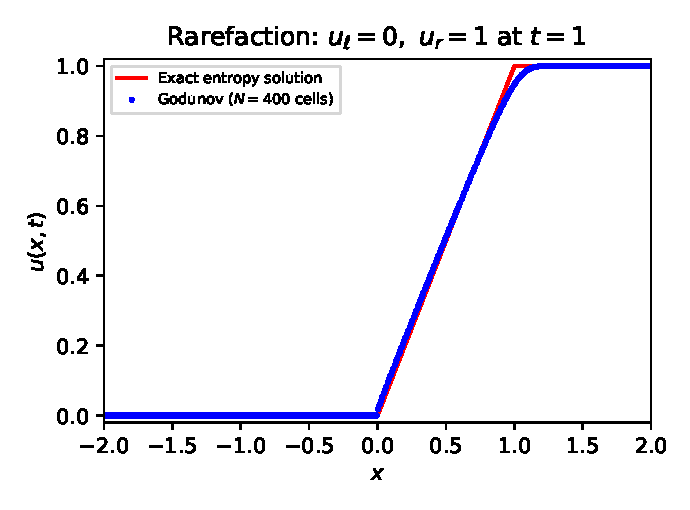
\includegraphics[width=0.44\textwidth]{figures/godunov_rarefaction.pdf}
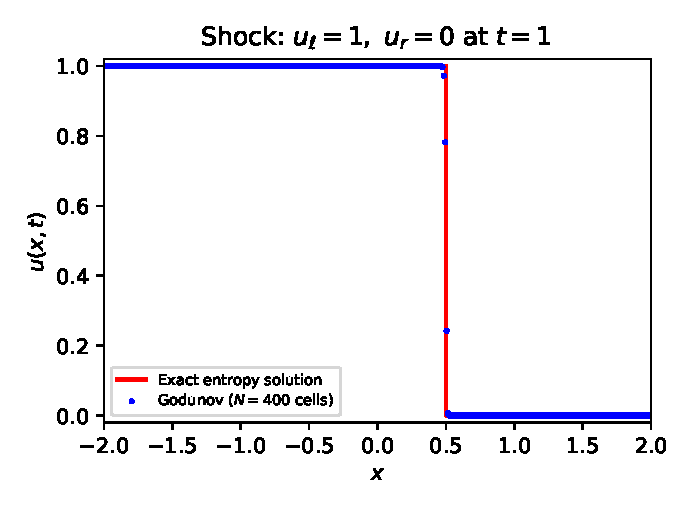
\includegraphics[width=0.44\textwidth]{figures/godunov_shock.pdf}
\caption{Godunov scheme (dots, $N=400$) against the exact entropy solution
(solid) at $t=1$. Left: rarefaction data $(0,1)$. Right: shock data
$(1,0)$.}
\label{fig:godunov-results}
\end{figure}

\begin{table}[h]
\centering
\begin{tabular}{r r r r r r}
  $N$ & $\Delta x$ & $L^1$ (rarefaction) & order & $L^1$ (shock) & order \\\hline
  200  & $2.0\times10^{-2}$ & $3.05\times10^{-2}$ & --- & $9.91\times10^{-3}$ & --- \\
  400  & $1.0\times10^{-2}$ & $1.82\times10^{-2}$ & 0.74 & $4.98\times10^{-3}$ & 0.99 \\
  800  & $5.0\times10^{-3}$ & $1.07\times10^{-2}$ & 0.77 & $2.50\times10^{-3}$ & 0.99 \\
  1600 & $2.5\times10^{-3}$ & $6.14\times10^{-3}$ & 0.80 & $1.24\times10^{-3}$ & 1.01 \\
  3200 & $1.25\times10^{-3}$ & $3.48\times10^{-3}$ & 0.82 & $6.23\times10^{-4}$ & 0.99 \\
  6400 & $6.25\times10^{-4}$ & $1.95\times10^{-3}$ & 0.84 & $3.13\times10^{-4}$ & 0.99
\end{tabular}
\caption{$L^1$ errors at $t=1$ and observed orders $\log_2(e_{N/2}/e_N)$.
All $N$ are multiples of $8$, so the shock lies on a cell interface.}
\label{tab:godunov-conv}
\end{table}

\paragraph{Shock.} The shock $x=st=0.5$ lies on a cell interface iff $8\mid N$,
and for such $N$ the error is $0.50\,\Delta x$ to two digits ($0.495$--$0.501$)
with observed order $\approx1$ (Table~\ref{tab:godunov-conv}). For
$N=97,\dots,103$ it ranges from $0.55\,\Delta x$ to $0.66\,\Delta x$
($0.655\,\Delta x$ at $N=100$, against $0.50\,\Delta x$ at $N=96,104$), so orders
computed between misaligned and aligned resolutions are unreliable ($N=100\to200$
would give $1.40$), which is why the table uses $N=200\cdot2^k$. In all cases the
error is proportional to $\Delta x$.

\paragraph{Rarefaction.} The error decreases monotonically, with observed orders
$0.74,0.77,0.80,0.82,0.84$ that are still increasing, so these experiments do not
establish a first-order rate. The error is confined to the fan region (outside
$[-0.2,1.2]$ it is below $3\times10^{-4}$ at $N=200$ and decays rapidly), but not
to the corners: for $N=200,\dots,6400$, the error on the fan interior
$0.2<x<0.8$, which carries about a third of the total, has observed orders
$0.75,0.79,0.81,0.83,0.85$, and the error within $0.1$ of the corners has orders
$0.65,0.70,0.75,0.79,0.81$, both rising. A corner effect alone therefore does not
account for the sub-first-order rate. One possible explanation is that the
numerical layers at the corners, of width $O(\sqrt{\Delta x})$, still overlap the
fan at these resolutions; this has not been tested.

\subsubsection{Numerical diffusion as vanishing viscosity}
\label{subsubsec:numerical-viscosity}

For the shock data the scheme is monotone, so by the discrete maximum principle
all states remain in $[0,1]$. All characteristic speeds are then nonnegative, so
the Godunov flux is the upwind flux $f(U_j^n)$, and the scheme reads
$U_j^{n+1}=U_j^n-\lambda(f(U_j^n)-f(U_{j-1}^n))$, $\lambda=\Delta t/\Delta x$.
Taylor expansion gives the modified equation
\begin{equation}
  \label{eq:modified-equation}
  u_t+u\,u_x=\frac{\Delta x}{2}\big(u(1-\lambda u)\,u_x\big)_x+O(\Delta x^2),
\end{equation}
a Burgers-type equation in conservative form, with state-dependent viscosity
$\nu(u)=\tfrac{\Delta x}2u(1-\lambda u)$, nonnegative exactly under
\eqref{eq:cfl}. Its travelling shock $1\to0$ of speed $\tfrac12$ satisfies
$\nu(u)u_\eta=\tfrac12u(u-1)$ in $\eta=x-t/2$; in units of $\Delta x$,
\begin{equation}
  \frac{du}{d\eta}=\frac{u-1}{1-\lambda u},\qquad
  \eta(u)=\eta_0+(1-\lambda)\ln(1-u)-\lambda u .
\end{equation}
The profile decays exponentially to $1$ as $\eta\to-\infty$ and reaches $0$ at
a finite $\eta_0$, which conservation of mass fixes as $\eta_0=1-\lambda/2$. The
$L^1$ distance from the sharp shock is then
\begin{equation}
  \frac{\|u-u_{\rm exact}\|_{L^1}}{\Delta x}
  =2\int_0^{u_0}\frac{u(1-\lambda u)}{1-u}\,du,\qquad
  (1-\lambda)\ln(1-u_0)-\lambda u_0=-\Big(1-\frac\lambda2\Big).
\end{equation}
Table~\ref{tab:numerical-viscosity} compares this with the measured shock
error on aligned grids, where $\lambda$ equals the CFL number since
$\max|U|=1$ (\texttt{code/numerical\_viscosity.py}).

\begin{table}[h]
\centering
\begin{tabular}{c c c c}
  CFL $=\lambda$ & measured ($N=1600$) & predicted & (pred.$-$meas.)/meas. \\\hline
  0.10 & 0.627 & 0.686 & $+9.4\%$ \\
  0.20 & 0.589 & 0.635 & $+7.8\%$ \\
  0.30 & 0.553 & 0.586 & $+6.0\%$ \\
  0.45 & 0.496 & 0.511 & $+3.0\%$ \\
  0.60 & 0.448 & 0.438 & $-2.2\%$ \\
  0.80 & 0.352 & 0.342 & $-2.8\%$ \\
  0.95 & 0.300 & 0.272 & $-9.3\%$
\end{tabular}
\caption{Shock $L^1$ error divided by $\Delta x$: measured (grids with
$8\mid N$) against the modified-equation prediction; the last column is computed from the tabulated values.}
\label{tab:numerical-viscosity}
\end{table}

The prediction is within about $3\%$ at CFL $0.45$ ($+3.0\%$) and within $10\%$
throughout, although the value at CFL $0.95$ is not yet asymptotic ($0.334$ at
$N=400$, $0.300$ at $N=1600$). Equating the error with the viscous-shock value
$4\ln2\,\nu_{\rm eff}$ of Proposition~\ref{prop:viscous-profile} ($s=\tfrac12$,
$\Delta=1$) defines an effective viscosity: the measured $0.50\,\Delta x$ gives
$\nu_{\rm eff}\approx0.180\,\Delta x$, the modified-equation profile gives
$0.184\,\Delta x$, and $\nu(\tfrac12)=\tfrac{\Delta x}2\cdot\tfrac12(1-\tfrac\lambda2)$
gives $0.194\,\Delta x$ at $\lambda=0.45$. Since $\nu_{\rm eff}=O(\Delta x)\to0$,
the scheme acts in the shock layer as a vanishing viscosity, in accordance with
Theorem~\ref{thm:vanishing-viscosity}; this is a consistency check rather than a
proof, as the numerical shock spans only a few cells and
\eqref{eq:modified-equation} omits the $O(\Delta x^2)$ terms.

\subsubsection{A consistent scheme that selects the wrong solution}
\label{subsubsec:non-entropy}

Consider the flux $\widehat f_{j+1/2}=f(U_j)$ if $\tfrac12(U_j+U_{j+1})>0$ and
$f(U_{j+1})$ otherwise, which is consistent and conservative but not monotone.
For the Riemann data $U_j=-1$ ($j\le0$), $U_j=+1$ ($j>0$) every numerical flux
equals $f(\pm1)=\tfrac12$, so $U^{n+1}=U^n$ exactly and the scheme returns the
stationary upward jump, the analogue for these data of $u_A$ in
Section~\ref{sec:nonuniqueness} (a weak solution by
\eqref{eq:rankine-hugoniot-burgers} with speed $0$, but not an entropy solution).
Godunov's flux at the same interface is $f(0)=0$, and the resulting scheme
produces instead the fan $u=x/t$ of Theorem~\ref{thm:riemann-solution}. At $t=1$ the $L^1(-2,2)$
distance to the entropy solution is $1.000$ for the non-monotone scheme for all
$N=200,400,800$, since $\int|\operatorname{sgn}x-\operatorname{clip}(x,-1,1)|\,dx=1$, while for
Godunov's scheme it is $6.1\times10^{-2}$, $3.6\times10^{-2}$,
$2.1\times10^{-2}$. By the Lax--Wendroff theorem \cite[Ch.~12]{leveque2002}
limits of consistent conservative schemes are weak solutions, so consistency and
conservation alone do not select the entropy solution: monotonicity
(Theorem~\ref{thm:godunov-convergence}) does.